\documentclass{template/openetcs_report}
% Use the option "nocc" if the document is not licensed under Creative Commons
%\documentclass[nocc]{template/openetcs_article}
\usepackage{lipsum,url}
\usepackage{supertabular}
\usepackage{multirow}
\usepackage{color, colortbl}
\usepackage{hyperref}
\usepackage{listings}
\usepackage{makeidx}
\definecolor{gray}{rgb}{0.8,0.8,0.8}
\usepackage[modulo]{lineno}

 \usepackage[acronym, % list of acronyms
  %section, % add the glossary to the table of content
            %description,% acronyms have a user-supplied description,
 style=longheader, % table style
 nonumberlist % no page number
  ]{glossaries}

\graphicspath{{./template/}{.}{./images/}}

\renewcommand*{\glspostdescription}{} %Deactivate point at the end of every description
\renewcommand*{\glossaryname}{Glossary}

%create glossary
 \makeglossaries
 %Glossary terms
 \loadglsentries{glossary}

\begin{document}
\frontmatter
\project{openETCS}

\newcommand{\define}[1]{\index{#1}\emph{#1}}






%Please do not change anything above this line
%============================

%user specified macros
%\input{sections/macros.tex}

% The document metadata is defined below

%assign a report number here
%\reportnum{OETCS/WP3/D3.5.1.3}

%define your workpackage here
\wp{Work-Package 3: ``Modeling''}

%set a title here
\title{openETCS System Architecture and Design Specification}

%set a subtitle here
\subtitle{Third iteration: Scope of openETCS ITEA2 Functions}

%set the date of the report here
\date{November 2014}


%document approval
%define the name and affiliation of the people involved in the documents approbation here
\creatorname{Baseliyos Jacob}
\creatorname{Jakob Gärtern}
\creatoraffil{DB Netz}

\techassessorname{[assessor name]}
\techassessoraffil{[affiliation]}

\qualityassessorname{Izaskun de la Torre}
\qualityassessoraffil{SQS}

\approvalname{Klaus-R\"udiger Hase}
\approvalaffil{DB Netz}


%define a list of authors and their affiliation here

\author{Baseliyos Jacob, Bernd Hekele}

\affiliation{DB Netz AG\\
  V\"olckerstrasse 5\\
  D-80959 M\"unchen Freimann, Germany}

\author{Marc Behrens}
\affiliation{DLR}

\author{David Mentre}
\affiliation{Mitsubishi Electric R\&D Centre Europe}

\author{Jos Holtzer, Jan Welvaarts, Vincent Nuhaan}
\affiliation{NS}

\author{Jacob G\"artner}
\affiliation{LEA Engineering}

% define the coverart
\coverart[width=350pt]{openETCS_EUPL}

%define the type of report
\reporttype{Architecture and Functional Specification}


\begin{abstract}
%define an abstract here
This document gives an introduction to the architecture of openETCS. The functional scope is tailored to cover the functionality required for the openETCS demonstration as a target of the ITEA2 project: the Utrecht Amsterdam use-case. It has to be read as an add-on to the models in SysML, Scade and to additional reading referenced from the document.
\end{abstract}

%=============================
\maketitle

%Modification history
%if you do not need a modification history table for your document simply comment out the eight lines below
%=============================


\chapter*{Modification History}
\tablefirsthead{
\hline 
\rowcolor{gray} 
Version & Section & Modification / Description & Author \\\hline}
\begin{supertabular}{| m{1.2cm} | m{1.5cm} | m{6.6cm} | m{3.7cm} |}
0.1 & Document & Initial document providing the structure & Baseliyos Jacob \\\hline
0.2 & Document & Workshop Results included and some pretty-printing & Bernd Hekele \\\hline

\end{supertabular}

% list subsubsections in table of contents
\setcounter{tocdepth}{3}


\tableofcontents
\listoffiguresandtables
\newpage
%=============================

%Uncomment the next line if you need line numbers for tracebility when the document is in review
%\linenumbers
%=============================


% The actual document starts below this line
%=============================

\mainmatter

\chapter{Introduction}

\section{Motivation}
The openETCS work package 3 (WP3) aims to provide – amongst others - the software architecture for the openETCS kernel in order to eventually build the software itself. WP3  partner has put great effort in the openETCS software design, thus far without making definite choices on the software architecture itself respective of functional breakdown and data structures of the openETCS kernel. Since the project planning foresees in the production of a reference software to be used as a demonstrator by June 2014, it is of paramount importance that a design freeze of the openETCS kernel architecture be finalized shortly but no later than November 2014.\\

In compliance with the agreements made during the last WP 3 meeting at the 10.09.2014 in Brussels, DB has taken the initiative to design the aforesaid architecture including of functional breakdown and data structures in order to safeguard a timely delivery of these products. Furthermore, DB has ensured that these developments are focused on including end user requirements so as to develop a design in conformity with the needs and requirements of the operators. Specialists of DB and NS have cooperated together with other partners in WP3 to produce this document.\\

As referred to above, the architecture description has to be finalized in the month of November 2014. This version of the document is a draft version, demonstrating the general directions and philosophy of the architectural design, the functional breakdown of the software and the data structures. The design is focused on maximum efficiency in order to maximize on RAMS performance of the end product.\\

\textbf{This document, named second iteration, is a draft document and will be developed until a complete architecture.}\\

Since this is a work in progress, any remarks referring to the improvement of the document, including reporting errors, are more than welcome. Any additional work done thus far on the subject by other WP3 partners will be incorporated in this document as long as it is aligned with and consistent or complementary  to the fundamental viewpoints advocated in this document after a review in respect to the openETCS process. At the same time, any contributions to the  integration of which will demand discussion or changes of the fundamentals as proposed in this document, will be discarded with . Only in this way the ITEA2 project is able to meet its objectives as mentioned above. There will be two workshops in which there is due time and opportunities to fine-tune this document and its contents. Any comments will be addressed there.\\

It is urgent to definitely finalize the architecture on a short notice and therefore this document will rather prescribe than describe the openETCS architecture, functional decomposition of the system and the data structures within the limits as stated above. The document is divided in two parts, i.e.:\\
•	A description of the general architecture of the openETCS OnBoard Kernel (software) including data structures prepared by NS….\\
•	A description of the functional decomposition of the openETCS OBU (software) in alignment with the general architecture prepared by DB…..\\


Furthermore, this document describes the preconditions on which said descriptions are based on, the status and planning of upcoming activities and the main objectives of DB and NS as the End User. Wherever necessary, reference will be made to documents that underline the agreements that have been made during the openETCS architecture design process and the activities and meetings of WP3. \\


\section{Objectives}

The prime objective of WP3 is to produce a rapid prototype for the openETCS reference system that can function as a demonstrator in collaboration with WP 4 and WP 5  for the openETCS approach and will be used as such in the final phase of the project. That phase is the first half of 2015.  This objective is defined as … 

\textbf{High level Objectives of this work:}\\
<<any further general statements on the ITEA2  objectives, like…>>\\
• Work on a model bases approach and process for effective collaborative work within an international ETCS developer team
as stated above, the project needs a definite architecture design by the end of 2014.  This document targets:\\
•	Defining the general design and conditions of the openETCS architecture, functional breakdown and data structures;\\
•	Providing the guidelines for discussion during the workshops that are planned in October and November 2014 that will result in the final and decisive version of this document;\\
•	Being the ‘platform’ for finalization i.e. whatever be the products or results of the workshops shall be integrated in this document. 
Apart from these general objectives, the document means to provide for the materials that will enable WP3 partners to improve the efficiency of the Work Package activities:\\
• The comprehensive architecture design shall enable splitting the work load according to the building blocks defined by the architecture and allocate strictly compartmented work parcels or activities to WP3 partners. \\
• Doing so will enable WP3 to avoid any double work\\
• Compartmenting the work load according to the functional building blocks as defined by the architecture will enable efficient planning of activities, be it individually or the integrated WP3 planning for the coming period, aiming at a just in time delivery of all results and products;\\
• Each partner that is responsible for one of the work parcels shall abide by the requirements in terms of quality and timeliness as defined by this document and prior documents and agreements made within the ITEA2 project.\\

\section{Roles, responsibilities and tasks}
In this section, the roles and responsibilities of the WP3 partners are confirmed, especially where they divert from what has been agreed upon at the start of WP3:\\
•	First of all, in the last WP 3 meeting in Brussels on  10.09.2014 DB proposed to take over the lead of the architecture design and functional breakdown. At the subsequent weekly scrum meeting on 12.09.2014,  it was agreed upon by all participants that DB will take over the lead (see Appendix … );\\
•\textbf{Planning:} Alstom as WP 3 leader will remain to be responsible for the planning and the allocation of the defined tasks to the different partners\\
•\textbf{Roles:} Alstom will also coordinate the work and safeguard that the defined results will be delivered according to the quality requirements that are agreed within the ITEA2 project and the schedule and the milestones that will be agreed upon during the coming workshops;\\
•All WP3 partners will deliver the results or products according to planning as will be agreed upon during the said workshops. \\

In the interest of a swift production of the critical documentation of which this version is a draft, specific tasks will be defined in terms of concrete results to be delivered, the timeframes in which these results must be produced and the partner who shall be responsible for that specific result and the planning. This is to safeguard the timely delivery. The process will be described in the next sections.\\

\section{Process}
\begin{itemize}
\item Alstom as WP 3 leader will be responsible for planning
\item Time and quality aspects should be respected
\item openETCS tools and methodology must be respected
\end{itemize}

Most of the operational requirements to WP3 in the last phases of the ITEA2 project have been described in the former paragraphs. This section will describe the process which has to lead to the final result: the reference software to be used in the demonstrator next year, more specifically the final description of the openETCS architecture including the data structures and its functional decomposition. The process will run as follows:\\
•	DB will supervise  the development of the first ‘firm’ draft of the specified products, ‘firm’ meaning that changes can only be made within the framework of these products and not to the fundamentals of these products as described in this document; \\
•	DB will supervise the preparation of the two workshops that are proposed by Alstom and aim at defining the final and definite architecture, data structures and functional decomposition. It will make proposals for a planning of the critical tasks that remain to be done;\\
•	Alstom will lead the two workshops following the preparations and the instructions of DB. Since all participants are intrinsically involved in the development work and tend to immerse themselves in technical discussions, for productivity purposes it is proposed to make use of a (non-technical) moderator that will be made responsible for coordinating the meeting, the discussions and the team efforts according ot the agenda.\\
•	Also for productivity reasons, introductory presentations will be restricted to the contents and setup of this document since all prior efforts have to be merged with this document and not the other way around. Following a general introduction into the work that has been so far, the other contributions will be scrutinized on their consistency with this document and any useful sections will be merged with this document.\\
•	During the workshops, there will be ample room reserved for enhancing this document, using other documents pertaining to the same field of work that have been delivered by other partners. Only material that is aligned with the general philosophy and structures proposed by this document, will be integrated;\\
•	In case conflicting views emerge over the benefits and value of certain contributions, at the very moment that parties conclude that they have conflicting views, these will be listed in an inventory for later discussion. The moderator shall note any such conflicts on the said inventory. Conflicting views will be treated at the end of each workshop whenever there is sufficient time or will be treated in a separate meeting that will be chaired by DB as coordinator of the ITEA2 project.\\
•	The workshop shall be attended by a secretary provided for by DB who is responsible for making the workshop minutes. Within a week after each workshop these minutes shall be distributed among the partners that have cooperated in the workshop and be reviewed by those. \\
•	The main objective of the workshops shall be the finalization of this document. In order to reach the specified result, the remaining tasks shall be identified and split into separate tasks or work parcels. Every task or work parcel will be allotted to one single responsible partner. Responsibility relates to the timely delivery of the defined result and according to quality requirements;\\
•	Alstom, as WP3 leader, will be responsible for the planning, allocation of tasks or work parcels to partners and will ensure timely delivery of results;\\
•	In case there will be tasks or work packages that cannot be finalized during the workshops or will be identified during the workshops and do not fit in the actual planning, these will be allotted in such a way that deadlines are perfectly clear and acknowledged by the party that is responsible for the results, fit within the general requirements of the project and are agreed upon in writing and executed by the responsible partners according to agreement;\\
•	DB as partner that has integral responsibility for both the ITEA2 project and responsible as well for the architecture etc. , is entitled to interfere take over the role as leader / coordinator in case the workshops prove to be insufficiently productive;\\
•	All output will be such, that it can be integrated in this document. It is the responsibility of DB to integrate the results and to deliver the final and definite version of this document. \\
•	The document concept will follow the openETCS process and tools (LaTex and Git-hub).\\

\section{Assumption and Preconditions}
\begin{itemize}
\item All future contributions shall be fully aligned an compliant the finalized and approved document 
\item Alls documents produced by the partners are requested to be compliant and merge to this document; other contributions will be discarded
\end{itemize}
The workshops are all about working as swift, as efficient and as productive as possible and make full use of the potential made available for these workshops by the partners. It is expected that the partners in the workshops will have the express intention to:\\
•	Contribute to the workshops with the intention to finalize the openETCS architecture;\\
•	Provide resources according to the agreements made prior to the Workshops;\\
•	Focus primarily on  getting concrete results regardless of methodological issues that might arise. Where necessary or opportune, classical project management methodology will be applied;\\
•	Provide full transparency with respect to experience, knowledge base and information touching the subjects to be treated in the workshops;\\
•	Document on paper or electronically all output of the workshops and integrate these with the underlying document;\\
•	Restrict discussions only to topics that have an immediate impact on the content or the quality of the end product: the improved version of this document.\\


\section{Functions ERTMS/ETCS}
The ERTMS / ETCS system was developed with a view to interoperability of trains on the 
different European rail networks. It is divided into "tracks" - and "board" finishes 
and shall establish a mutual message operation, by beacons or through a "radio" - 
The transmission system (in this case a mobile telephone network GSM-R) is performed. 
It defines several operating levels, and the system must also interfaces with the 
existing monitoring systems of the trains (using \gls{STM}) have. 
The ERTMS / ETCS system provides the transport operator (the track) the choice of conditions 
concerning the use and operation. 
The train must therefore may go with different operating conditions on routes. 
Thus has the onboard equipment but must be implemented, 
to the interoperability of the train to ensure on the other networks. 
These functions must therefore correspond to one standard: the \gls{SRS} (version 3.3.0). 

application functions, which have two different species of origin: 
defined in the \gls{SRS}: here one finds in particular the 
speed monitoring- and transfer functions; these functions 
must be implemented in full accordance with the \gls{SRS}; they can in 
indeed be on any network on which the train is used; these functions 
are described below in Section \ref{SRSFunction}; 


Moreover, there are functions to adapt to the train: so, for example, the processing 
a "separation distance" in the airborne equipment trigger: 
This is dependent on the distribution of functions between the 
Control monitoring equipment (which the ERTMS / ETCS), and the other 
CCS Systems.

\section{openETCS Architecture: History and Iterations}

The openETCS Architecture and Design is implemented in iterations \cite{deployment}. The current step (second iteration) is based on a step to implement the kernel functions of the ETCS system \cite{firstIteration}. For a better understanding of the scope the Iteration is described in the following.

\subsection{First Iteration Functional Scope: The Minimum OBU Kernel Function}
\label{sec:FunctionalScopeTheMinimumOBUKernelFunction}

The openETCS first iteration architecture and the design of the openETCS OBU software as mainly specified in \cite{subset-026} UNISIG Subset\_026 version\_3.3.0. 

The appropriate functionality has been divided into a list of functions of different complexity (see the WP3 function list \cite{functions}).

All these functions are object of the openETCS project and have to be analysed from their requirements and subsequently modelled and implemented. With limited manpower, a reasonable selection and order of these functions is required for the practical work that allows the distribution of the workload, more openETCS participants to join and leads to an executable---limited---kernel function as soon as possible. 

While the first version of this document focuses on the first version of the limited kernel function, it is intended to grow in parallel to the growing openETCS software.

The first objective of the first iteration was
\begin{itemize}
	\item ``Make the train run as soon as possible, with a very minimum functionality, and in the form of a rapid prototype.''
\end{itemize}
This does not contradict the openETCS goal to conform to EN50128.
\begin{itemize}
	\item After a phase of prototyping, the openETCS software shall be implemented in compliance to EN50128 for SIL4 systems.
\end{itemize}

\subsection{How to find the functions of the First Iteration in the Architecture}
The functions will be merged with the new architecture. Wherever a function has already been in the scope it will be marked as "first iteration".

%\section{Glossary and Abbreviations}
%\glossarystyle{long}
%\printglossary[title=]


%\section{Abbreviations}
%\printglossary[type=\acronymtype,title=]

\glsaddall
\printglossaries


\section{Data dictionary}
\textbf{concept for the data dictionary ...}\\

\chapter{Input Documents}
See Wiki page on ....

\textbf{https://github.com/openETCS/modeling/wiki/Input-Documents-Repository}\\


\chapter{Product Backlog}
\textbf{See on:}\\ 


\chapter{Architecture description (by layers)}

\section{Introduction to the Architecture}

\subsection{Abstract Hardware Architecture}

For proper understanding of openETCS \gls{API} and of constraints imposed on
both sides of the \gls{API}, we need to define a \define{reference abstract hardware architecture}. This hardware architecture is ``abstract''
is the sense that the actual vendor specific hardware architecture
might be totally different of the abstract architecture described in
this chapter. For example, several units might be grouped together on
the same processor.

However the actual vendor specific architecture shall fulfil all the
requirements and constraints of this reference abstract hardware
architecture and shall not request additional constraints.

\subsection{Definition of the reference abstract hardware architecture}

\begin{figure}
  \centering
  \includegraphics[width=\linewidth]{abstract-hardware-architecture.pdf}
  \caption{Reference abstract hardware architecture}
  \label{fig:hardware-arch}
\end{figure}

The reference abstract hardware architecture is shown in figure
\ref{fig:hardware-arch}.

The reference abstract hardware architecture is made of a bus on which
are connected \define{units} defining the \gls{OBU}:

\begin{itemize}
\item \gls{EVC};
\item \gls{TIU};
\item \gls{ODO};
\item \gls{DMI};
\item \gls{STM};
\item \gls{BTM};
\item \gls{LTM}: Not part of this openETCS implementation;
\item EURORADIO;
\item \gls{JRU}: Not part of this openETCS implementation;
\end{itemize}

Elements not being part of this implementation are marked. 

Those units shall working concurrently. They shall exchange
information with other units through asynchronous message passing.

\subsection{Reference abstract software architecture}
\label{software-arch}

\begin{figure}[htbp]
  \centering
  \includegraphics[width=\linewidth]{software-architecture.pdf}
  \caption{Reference abstract software architecture}
  \label{fig:software-arch}
\end{figure}

The \define{reference abstract software architecture} is shown in figure
\ref{fig:software-arch}. This architecture is made of following
elements:
\begin{itemize}
\item \define{openETCS executable model} produced by the
  \cite{scade-model} Scade Model. It shall contain the program implementing core
  ETCS functions;
\item\define{openETCS model run-time system} shall help the execution
  of the openETCS executable model by providing additional functions
  like encode/decode messages, proper execution of the model through
  appropriate scheduling, re-order or prioritize messages, etc. 
\item \define{Vendor specific \gls{API} adapter} shall make the link between
  the Vendor specific platform and the openETCS model run-time system.
  It can buffer message parts, encode/decode messages, route messages
  to other \gls{EVC} components, etc.
\item All above three elements shall be included in the \gls{EVC};
\item \define{Vendor specific platform} shall be all other elements of
  the system, bus and other units, as shown in figure
  \ref{fig:hardware-arch}.
\end{itemize}

We have thus three interfaces:
\begin{itemize}
\item \define{model interface}
 is the interface between openETCS
  executable model and openETCS model run-time system. 
\item \define{openETCS \gls{API}}
 is the interface between openETCS model
  run-time system and Vendor specific \gls{API} adapter.
\item \define{Vendor specific \gls{API}}
 is the interface between Vendor
  specific \gls{API} adapter and Vendor specific platform. This interface is
  not publicly described for all vendors. You can find the Alstom imnplementation as an example.
\end{itemize}

The two blocks openETCS executable model and openETCS model run-time
system are making the \define{Application software} part. This Application software might be either openETCS reference software or
vendor specific software.

The Vendor specific \gls{API} adapter is making the \define{Basic software} part.


\section{Functional breakdown}

\subsection{F1: openETCS \gls{API} Runtime System and Input to the EVC)}
%Authors: Bernd Hekele (DB)

\begin{figure}[hbtp]
\centering
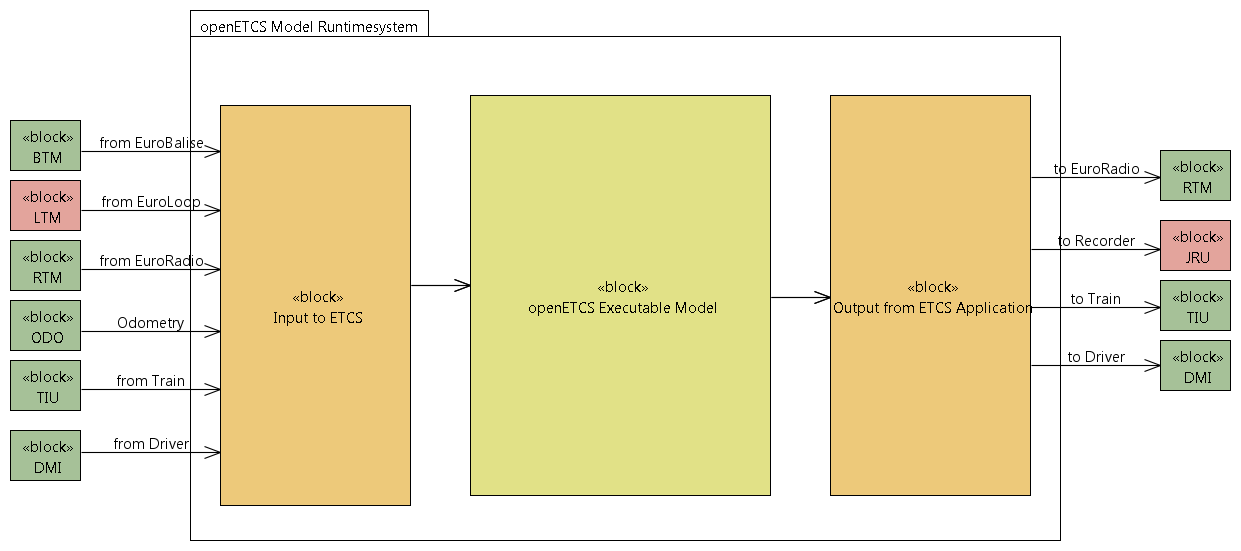
\includegraphics[width=\linewidth]{openETCSAPI.png}
\caption{openETCS API Highlevel View}
\label{fig:apiHighLevel}
\end{figure}

Figure \ref{fig:apiHighLevel} shows the structure of API with respect of the software architecxture. Input boxes and output boxes not implemented in this stage are marked as red, other interfaces are marked as green. The System covers functions for processing Inputs from other Units, functions for processing Outputs to other functions and a basic runtime system. Inputs are used to feed the input to the executable model before calling it, outputs are used for collecting information provided by the executable model to be passed to the relevant interfaces after the execution cycle has finished.

\subsubsection{Principles for Interfaces (openETCS \gls{API})}


Information  is exchanged \define{messages} in an asynchronous way. A message is a set
of information corresponding to an event of a particular unit, e.g. a
balise received from the \gls{BTM}. The possible kind of messages are
described in chapter \ref{information-flows}.

The information is passed to the executable model as parmeters to the snychronous call of a procedure (Interface to the executable model). Since the availability of input messages to the application is not guaranteed the parts of the interfaces are defined with a "present" flag. In addition, fields of input arraysquite often is of variable size. Implementation in the concrete interface in this use-case is the use of a "size" parameter and a "valid"-flag.


\subsubsection{openETCS Model Runtime System}
The openETCS model runtime system also provides:

\begin{itemize}
\item Input Functions From other Units\\
In this entity messages from other connected units are received.
\item Output Functions to other Units\\
The entity writes messages to other connected units.
\item Conversation Functions for Messages (Bitwalker)\\
The conversion function are triggered by Input and Ouput Functions. The main task is to convert input messages from an bit-packed format into logical ETCS messages (the ETCS language) and Output messages from Logical into a bit-packed format. The logical format of the messages is defined for all used types in the openETCS data dictonary. \\
Variable size elements in the Messages are converted to fixed length arrays with an used elements indicator.\\
Optional elements are indicated with an valid flag.
The conversion routines are responsible for checking the data received is valid. If  faults are detected the information is passed to the openETCS executable model for further reaction. 
\item Model Cycle\\
The executable model is called in cycles. In the cycle 
\begin{itemize}
\item First the received input messages are decoded
\item The input data is passed to the executable model in a predefined order. \textbf{(Details for the interface to be defined)}.
\item Output is encoded according to the \gls{SRS} and passed to the  buffers to the units.
\end{itemize}
\end{itemize}


\subsubsection{Input Interfaces of the openETCS API From other Units of the OBU}

\tablefirsthead{
\hline 
\rowcolor{gray} 
Unit & Name & Number & Processing Function & Description \\\hline}
%\begin{supertabular}{| m{1.2cm} | m{1.5cm} | m{1.2cm} | m{3.7cm}  | m{3.7cm} |}
\begin{supertabular}{| c | c | c | c  | c |}
\gls{BTM} & Balise Telegram & 0..1 & Receive Messages & \\\hline
\gls{DMI} \\\hline
EURORADIO & Communication Management  & 0..1 & Communication Management & \\\hline
EURORADIO & Radio Messages & 0..1 & Receive Messages & \\\hline
\gls{ODO} & Odometer & 1 & All Parts & \\\hline
Startup \\\hline
TIU & Train Data & 1 & All Parts & \\\hline
\end{supertabular}

The following list gives an more detailed overview of the structure of the interfaces:

List of Packets Received:


Radio Messages

Outputs:\\
\subsubsection{Output Interfaces of the openETCS API TO other Units of the OBU}

\tablefirsthead{
\hline 
\rowcolor{gray} 
From Function & Name &  To Unit & Description \\\hline}
%\begin{supertabular}{| m{1.2cm} | m{1.5cm} | m{1.2cm} | m{3.7cm}  | m{3.7cm} |}
\begin{supertabular}{| c | c | c | c  | c |}
 & Radio Output Message & \ EURORADIO & \\\hline
 & Communication Management  &  EURORADIO  & \\\hline
 & Driver Information & \gls{DMI} \\\hline
 & Train Data  & TIU &  \\\hline
\end{supertabular}

Packets:
to be completed

Radio Messages
to be completed
 
\subsection{Receive msg´s/ check consistency}
\subsubsection{Short Description of Functionality}

The block ``Receive msg's / check consistency'' is responsible for receiving Eurobalise-telegrams and Euroradio-messages from the API and perform several consistency checks on this input.

The block collects the telegrams of balises in order to build balise group messages. Euroradio messages are always delivered as a whole message. After receiving, building and checking a message, the message is delivered to the output of the module for further processing by other modules.

% - version management (should be part of the bitwalker)\\
% - management of duplicated balises (should be part of the bitwalker)\\
% - management of multiple received balises (should be part of the bitwalker)\\
% - build BG-messages\\
% - Determine passing direction\\
% - Store passing direction if received from RBC\\
% - Store radio messages\\
% - check linking consistency and delete detected and missed BG's from announced BG's\\
% - check BG-message consistency\\
% - check Radio-message consistency\\
% - Retrieve individual packets (for delivery to filtering)\\

\subsubsection{Input}
\framebox{Note: Only radio functionality covered}

The input of the module is originated from the openETCS-API. The API is described in \cite{alstom-api}.

For delivering messages received by the EURORADIO module to the application software, the services \texttt{WRITE\_RTM\_MESSAGE} and \texttt{WRITE\_RTM\_EMERGENCY\_MESSAGE} are defined (see 4.14.6 in \cite{alstom-api}).

For the current iteration, emergency messages are not relevant.\\The API-service \texttt{WRITE\_RTM\_EMERGENCY\_MESSAGE} will not be implemented.

The service \texttt{WRITE\_RTM\_MESSAGE} has one parameter:
\begin{itemize}
 \item \texttt{THE\_RTM\_MESSAGE}: Input of type \texttt{API\_TYPES.RTM\_IN\_MESSAGE\_T}
\end{itemize}

The type \texttt{RTM\_IN\_MESSAGE\_T}  is used for normal messages, which can contain connection confirmations, information about connection problems or data.

\begin{tabular}{| c | l | l | l |}
 \hline
 \textbf{Index} & \textbf{Element name} & \textbf{Element type} & \textbf{Description}\\ \hline
 0 & RADIO\_DEVICE & ETCS\_ID\_T & Source interface of the message\\
 1 & REASON & RTM\_DIAGNOSTIC\_CODE\_T & Diagnostic code for connection problems\\
 2 & DATA & RTM\_MESSAGE\_T & Decoded message, CRC-checked\\
 \hline
\end{tabular}

\textbf{TODO:} Balise-channel

% A Eurobalise telegram consists of several fields shown in the table below. The table is an excerpt from the SRS, chapter 8.4.2.1. In this chapter the description of the fields can be found.
%  
%  
%  \begin{tabular}{| c | l | c  |}
%   \hline
%   \textbf{Field No.} & \textbf{VARIABLE} & \textbf{Length (bits)} \\ \hline
%   1 & Q\_UPDOWN & 1\\
%   2 & M\_VERSION & 7\\
%   3 & Q\_MEDIA & 1\\
%   4 & N\_PIG & 3\\
%   5 & N\_TOTAL & 3\\
%   6 & M\_DUP & 2\\
%   7 & M\_MCOUNT & 8\\
%   8 & NID\_C & 10\\
%   9 & NID\_BG & 14\\
%   10 & Q\_LINK & 1\\
%   \textit{-} & \textit{Packet 0 (Virtual balise cover) (optional)} & \textit{14}\\
%   \textit{-} & Information & variable\\
%   \textit{-} & Packet 255 & 8\\  
%   \hline
%  \end{tabular}
%  
%  \textbf{Relevant messages for track Utrecht-Amsterdam:} packets from balises: 3, 41, 42, 45, 46, 65, 72, 137, 255
%  
 


% \begin{itemize}
%  \item packets from balises: 3, 41, 42, 45, 46, 65, 72, 137, 255
% \end{itemize}
% \item unchecked Euroradio message
 \begin{itemize}
  \item messages from rbc: 2, 3, 6, 8, 15, 24, 27, 32, 39, 41
  \item packets from rbc: 3, 5, 15, 21, 27, 41, 42, 57, 58, 65, 68, 72, 80
 \end{itemize}
%\end{itemize}


\subsubsection{Output}
\framebox{Note: Only radio functionality covered}

The module produces the input-data for the Filtering (Mode/Level) module. The Filtering (Mode/Level)-module expects the messages received either via Euroradio or Eurobalise. The message is transmitted unchanged, if all consistency checks were successful.

Further outputs are the status information of the radio and a output-channel for acknowledgment- and rejection-messages to the RBC.

An Euroradio message from track to train consists of several fields shown in the table below. The table is an excerpt from the SRS, chapter 8.4.4.6.1. In this chapter the description of the fields can be found.

  \begin{tabular}{| c | l |}
  \hline
  \textbf{Field No.} & \textbf{VARIABLE}\\ \hline
  1 & NID\_MESSAGE\\
  2 & L\_MESSAGE\\
  3 & T\_TRAIN\\
  4 & M\_ACK\\
  5 & NID\_LRBG\\
  - & variables as required by NID\_MESSAGE\\
  - & packets as required by NID\_MESSAGE\\
  - & Optional packets\\
  - & Padding\\
  
  \hline
\end{tabular}

\subsubsection{Data}

An internal data structure to temporarily store balise telegrams for building messages is needed.

\subsubsection{Reference to the SRS (or other requirements)}
\framebox{Note: Only radio functionality covered}

\paragraph{Euroradio}
\begin{itemize}
 \item SRS subset 26, chapter 8.4.4: Rules for Euroradio messages
 \item SRS subset 26, chapter 3.16: Data consistency
\end{itemize}


\subsubsection{Functionality}
\framebox{Note: Only radio functionality covered}
\subparagraph{Receive Euroradio from API}
The first stage of the module is the reception of Euroradio-messages and Eurobalise-Telegrams from the openETCS-API. At each cycle the following conditions can occur:
\begin{enumerate}
 \item No new Euroradio-message or Eurobalise-telegram is available.
 \item A new Euroradio-message is available
 \item A new Eurobalise-telegram is available
 \item A new Euroradio-message and a new Eurobalise-telegram is available.
\end{enumerate}

\paragraph{Content checks}
\begin{itemize}
 \item The computed length of the message must be equal to the value in \texttt{L\_MESSAGE}. (SRS 8.4.4.2.1)
 \item The whole message must be complete and contains all necessary fields. (SRS 8.16.1.1)
 \item The message must respect the ETCS language. (SRS 8.16.1.1)
 \item The variables of the message does not contain invalid values. (SRS 8.16.1.1) \\\textbf{TODO:} Check value range? Or is the bitwalker already checking?
 \item Check if the specified priority of message is equal to the priority with which the message was received. (SRS 3.16.3.1.3.1)
\end{itemize}


\paragraph{Timing checks}
\begin{itemize}
 \item Check if the timestamp of a message is greater than the timestamp of the former message (SRS 3.16.3.3.3)
 \item If a message contains the timestamp ``Unknown'', check if this message is part of the initiation of the communication session. (SRS 3.16.3.3.4)
 \item Perform the check with the current packet $n$:  $T\_TRAIN_{n} <= T\_TRAIN_{n-1} + T\_NVCONTACT$ (SRS 3.16.1.1). This ensures, that the packet was received in due time.
\end{itemize}

\paragraph{Actions for inconsistent messages}
\begin{itemize}
  \item If a message is not consistent, it shall be rejected. (SRS 3.16.3.1.1.1)
  \item The RBC shall be informed, when a message was rejected (SRS 3.16.3.1.1.2). Therefore an error report must be sent (packet number 4). 
  \item If the RBC requested an ACK for a received message, the ACK shall be sent. (SRS 3.16.3.5)
\end{itemize}

The check by the Euroradio-protocol (3.16.3.1.1) will not be performed by the model, but on a lower level (RTM or openETCS-API).

Safe connection supervision is not in the scope of this module. This functionality will be implemented by the ``Manage Radio communication'' module. The ``Receive message and check consistency''-module will provide the necessary status data about the connection as an output.

% a bit more structured

\subsection{Build coordinate system and calculate train position}
- Update the coordinate system when a new \gls{BG} is detected (taking into account detected “balise 1” from not completed \gls{BG}'s), i.e. backward -   - Calculation of position of passed \gls{BG}'s.\\
- Management of multiple detected \gls{BG}'s\\
- Relate the (location based) information in received messages to the reference system\\
- Update train position at LR\gls{BG}\\
- Update the train position with the distance driven since last update (or reset to LR\gls{BG} position)\\

\subsection{Store inputs from the TIU}
- Store status inputs (sleeping indicator etc.)\\
- Store changed train data\\
- Store brake status (e.g. in the handling of brake testing).\\
- Store status of on-board systems (for displaying to the driver)\\
- Isolation\\
- Passive shunting\\

\subsection{Store inputs from the \gls{DMI}}
- Store received acknowledgement and inputs in the “\gls{DMI} request buffer” (includes “data-entry”)\\

\subsection{Filtering (Mode/Level) - One packet per type}
\textbf{ISSUE: HOW MANY PKT 44, 65 AND 66 PER MESSAGE ARE MAXIMALLY SUPPORTED?}\\
- Check on announced and immediate level transition orders in the messages to be filtered (needed for further criteria for filtering, to decide if the data shall be stored in the transition buffer).\\
- Filter data stored in the transition buffer according to the current level (what to do if similar information is available in the new message??). Data can be rejected, accepted or kept in the transition buffer.
(Filtering according to new level will be done directly afterwards in the next cycle)\\
- Filter new received messages according to the current level (new level will be done in the next cycle as according to \gls{SRS} data first has to be filtered according to old level and afterwards to new level). Data can be rejected, accepted or stored in the transition buffer.\\
- Filter (level) accepted data according to originating RBC (supervising or other). Information from \gls{BG}'s, loops or RIU is not filtered with this filter.\\
- Filter (level and RBC) accepted data according to the current mode (only reject or accept)\\

\subsection{Store data (direct orders, \gls{BG} lists, NV, track data, procedure parameters, confirmations)}
- Store direct and conditional orders\\
- Store \gls{BG} lists for SH and SR\\
- Store National Values, including procedure status information\\
- Store new received track data (version, etc.)\\
- Store procedure parameters\\

\subsection{Update location based data structures}
- Overwrite location based data from a given location on-wards (reference location given in the message)\\
- Insert “Locations” in the data structure, in the order the “Locations” will be passed.\\

\subsection{Manage specific location based data:}
- movement authority (MA) list of sections, message 37, packet 12 (level 1), message 3, packet 15 (level 2), 16 (repositioning, i.e. extending the current section), message 33 (??), packet 70 (route suitability), message 9 (request to shorten MA), packet 90 (track ahead free leads to MA request)    minimum number of elements to be stored: 6\\
- list of announced \gls{BG}'s linking information: packet 5  minimum number of elements to be stored: 30\\
- adhesion factor: packet 71;  only one element\\
- the “gradient profile” (in: pkt 21)  minimum number of elements to be stored: 50\\
- Speed profiles:  packet 27 (SSP)  (the worst case can be determined at reception)\\
- Packet 13	minimum number of elements to be stored: 50\\
- Speed restrictions and non-continuous speed profiles: packet 51 (axle load profile), packet 52 (permitted braking distance), packets 65/66 (TSR), packet 88 (level crossing, incl. stop condition to be reset at standstill). 
minimum number of elements to be stored: TSR: 30, axle load: 30, permitted braking distance:  5 , level crossing: 10. \\
- Reversing area's: packets 138, 139	minimum number of elements to be stored: 1\\
- Mode dependent speeds: message 2  and packet 80  minimum number of elements to be stored: 6\\
- Level transitions: packet 41  minimum number of elements to be stored:  (see ss26, 5.10.1.6): 1\\
- RBC transitions: packet 131\\
- Radio infill area entry or exit: packet 133\\
- Loop announcement: packet 134\\
- \gls{DMI} information: packets 72,76 (text messages), packet 79 (geographical position information), message 34 (track ahead free request)  minimum number of elements to be stored: fixed text: 5, free text: 5, geographical position: \\
- Track conditions (to be passed to the TIU and displayed at the \gls{DMI}): packet 39 (traction system), packet 40 (current limitation),  packet 68 (diverse track conditions), packet 69 (platform conditions). Pkt 139  minimum number of elements to be stored: 20, + 1 for change power supply + 1 for platform conditions, + 1 for current limitation\\
- Route suitability: minimum number of elements to be stored: 3\\
- Big Metal Mass: Technical information (to be used for \gls{BG}-filtering): packet 67 (ignore \gls{BG} integrity)  minimum number of elements to be stored: 5\\
- Virtual balise covers:  minimum number of elements to be stored: 10\\
- list of position report locations. In: pkt. 58  minimum number of elements to be stored: 15\\
- Announced national values.  In: pkt 3 minimum number of elements to be stored: 1
- If new national values are announced, then those can lead to more restrictive braking curves. Therefore a speed restriction has to be calculated for the location where the values become valid, based on the targets in advance of this point. \\

\subsection{Build and update MRSP and list of targets at LR\gls{BG}}
- Overlay speed restrictions (one by one) over the resulting SSP as received from “build location based data”.\\
- Close the resulting profile with the “end of authority” or “limit of authority” as delivered by “MA-management” resulting in the MRSP at the LR\gls{BG}.
(in on-sight or limited supervision mode, those may not be available)\\
- Select list of “speed reductions”\\
- Evaluate (backwards) which targets are relevant, resulting in the list of most restrictive targets at the LR\gls{BG}.\\
- Relocate targets (beyond this location) to the “minimum border crossing location”, i.e. the minimum safe location where National values are changed, and add the minimum resulting speed at this location to the list of targets.\\
- Reasoning:  new national values might cause more conservative braking curves which otherwise could lead to an intervention at the border.\\

\subsection{Profile supervision, i.e. BCM and ceiling speed supervision (active for FS, OS and LS)}
- Update MRSP for distance driven, i.e. lower the distance to all speed decreases with the maximum distance driven since last update, lower the distance to all speed increases with the minimum distance driven since last update, reorder the distances in the list if locations to lower and to increase changed order.\\
- Determine the local maximum speed\\
- Update the list of targets, i.e. lower the distance to all targets with the maximum distance driven since last update (order will not change) and select the current most restrictive target (always the first in the list)\\
- braking curve monitoring; calculate the braking curves to the most restrictive target, taking into account gradients\\
- ceiling speed supervision; monitor against the local maximum speed.\\

\subsubsection{Movement supervision}
- Roll away protection\\

\subsubsection{Area Supervision}
In shunting, post trip, reversing and staff responsible an area (plus in some cases ceiling speed) is protected. In unfitted only a speed. The way the area is protected differs per mode therefore a function shall be available for each mode:\\
- area supervision in shunting (taking into account a list of \gls{BG}'s to be passed)\\
- area supervision in staff responsible (taking into account a list of \gls{BG}'s to be passed and/or a distance)\\
- reversing area supervision\\
- post trip supervision (only reverse movement).\\

\subsubsection{Update procedure status (including commanding actions towards driver, radio or RBC)}
- SoM:\\ 
- EoM\\
- Enter shunting by driver or track side command
override\\
- Enter “on sight”\\ 
- Enter “staff responsible”\\
- level transitions\\
- Manage train trip\\
- Exit shunting\\
- Passive shunting\\
- Change train orientation\\
- Splitting/combining\\
- Stopping in rear of LX level crossing\\
- Changing train data (not by the driver)\\
- Handling track conditions (including indications):  not applicable for Amsterdam-Utrecht\\
- Limited supervision entry:  not applicable for Amsterdam-Utrecht\\
- release brakes (after trip)\\
- handle track ahead free request\\

\subsubsection{Mode/Level management}
- Manage all conditions for level changes except the direct transitions (handled in filtering): F41\\
- Manage all conditions for mode changes (except msg 16 if that leads to a mode change): F42\\

\subsubsection{\gls{DMI} management}
- update the MRSP at the LR\gls{BG} and construct the \gls{DMI} image\\
- collect BCM results\\
- Check displaying of location dependent txt messages\\
- Calculate geographical position based on stored track-km references\\
- Display required ack-requests, T.A.F. requests etc.\\
- Display mode and level information\\

\subsubsection{RBC communication}
- Manage confirmation requests.\\
- Report train position\\
- sent train data for validation\\
- provide acknowledgements on data reception\\

\subsubsection{TIU communication}
- Communicate track conditions\\
- Brake test procedure.\\

\subsubsection{JRU and \gls{STM} management: not applicable for Utrecht-Amsterdam}

\newpage
\subsection{Filter Track informationen}

\subsubsection{Interfaces}
\textbf{Input from:} Receive MSG Check Consistency and Coordinate System and Train Position\\
\textbf{Output to:} Build Data structure and Location Based/ Build Data Structures Drivers\\
\begin{figure}[hbtp]
\centering
\includegraphics[scale=0.7]{images/FilterInandOUt}
\caption{Filter In and out}
\end{figure}

\subsubsection{SysML Model}
\begin{figure}[hbtp]
\centering
\includegraphics [scale=0.5]{images/SysMLFilter}
\caption{SysML Filter}
\end{figure}

\chapter{Design description}


\section{Detailed functional description}
\textbf{Reference to \gls{SRS}: § 4.8.1, § 4.8.2, § 4.8.3, § 4.8.4}\\

\section{Documentation of design}
§ 4.8.1.6 Messages will be buffered, if...\\

\begin{figure}[hbtp]
\centering
\includegraphics [scale=0.7]{images/Decisionsonfilter}
\caption{Decision}
\end{figure}
 \newpage

\section{SCADE Model}





 
\appendix

\bibliographystyle{unsrt}
\bibliography{architecture}

\newpage
\addcontentsline{toc}{chapter}{Index}

\printindex

%===================================================
%Do NOT change anything below this line

\end{document}

